\documentclass[a4paper]{article}

\usepackage[utf8]{inputenc}
\usepackage[english]{babel}

\usepackage{amsmath,amsthm,amssymb}
\usepackage{geometry} % for correct margins
\usepackage{graphicx}
\usepackage{listings}
\usepackage{hyperref}

\newcommand{\prog}[1]{\texttt{#1}}
\newcommand{\pfun}[1]{\textsf{#1}}

\lstset{basicstyle=\ttfamily,
language=C,
}

\title{Concurrency Theory, Assignment Lecture 10}
\author{Krasimir Georgiev}

\begin{document}
\maketitle

The following PSF specification
\href{https://github.com/comco/concurrency-theory-assignments/tree/master/assignment-lecture-10/Factory.psf}{\texttt{Factory.psf}}
correctly models the manufacturing process and has a correct animation.

\begin{enumerate}
    \item The use of the unbounded queue \prog{WC6} in the modelling of the
        processing of products between work cells \prog{WC3} and \prog{WC4} is
        convenient, but unrealistic. There is the obvious practical issue of
        limited space; in reality the factory can have a mode of operation in
        which an unbounded space is really necessary; thus a limited-depth queue
        would be a more precise model of the interaction because it doesn't hide
        the potential deadlock that might occur from the overflow the queue.

    \item Since the way the simulation interprets actions as strings, it cannot
        distinguish between actions of the same name, so \emph{in the animation
        it looks like} 2 copies of the product \prog{A} occupy the same work
        cell, whereas \emph{they occupy the two copies of} \prog{WC2}.

        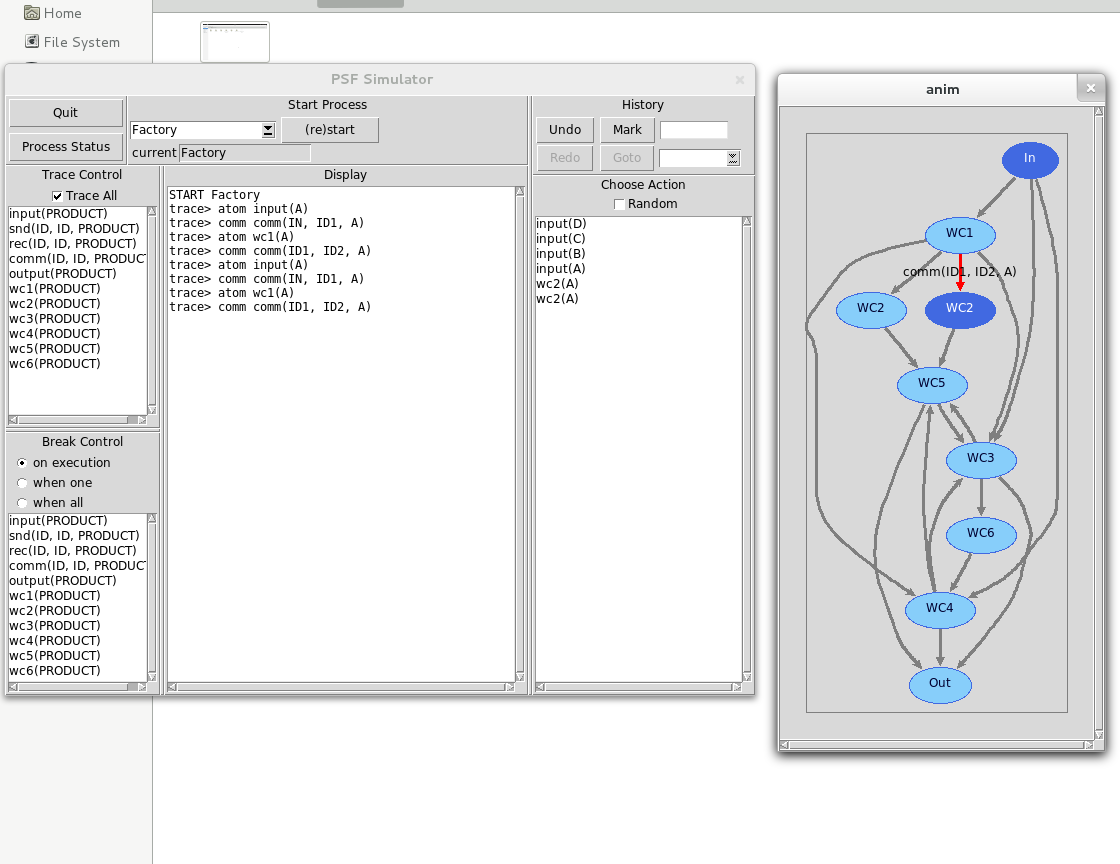
\includegraphics[scale=0.3]{animation-merged-1.png}

    \item A possible solution is implemented in \texttt{Factory.psf}. There, a
        separate work cell \prog{WC2p} is derived from \prog{WC2}, having
        parallel definition using the new atom \prog{wc2p} and the new ID
        \prog{ID2p}. The implementation of work cells \prog{WC1} and \prog{WC5}
        needs to be updated accordingly. The following image illustrates the
        situation from before:

        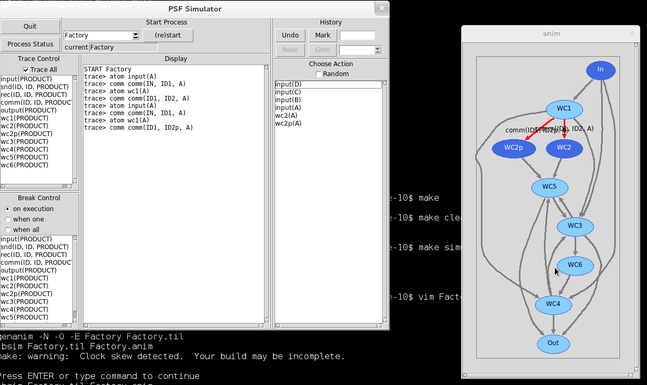
\includegraphics[scale=0.5]{animation-splitted-1.png}
\end{enumerate}

The source code of this assignment can be found on
\href{https://github.com/comco/concurrency-theory-assignments/tree/master/assignment-lecture-10}{GitHub}.
\end{document}
